%==============================================================================
% Sjabloon onderzoeksvoorstel bachproef
%==============================================================================
% Gebaseerd op document class `hogent-article'
% zie <https://github.com/HoGentTIN/latex-hogent-article>

% Voor een voorstel in het Engels: voeg de documentclass-optie [english] toe.
% Let op: kan enkel na toestemming van de bachelorproefcoördinator!
\documentclass{hogent-article}
\usepackage{graphicx}
\usepackage[most]{tcolorbox}
\definecolor{probkleur}{RGB}{255,255,150}   % lichtgeel
\definecolor{hoofdkleur}{RGB}{180,255,180}% lichtgroen
\definecolor{probleemdomein}{RGB}{180,200,255} % lichtblauw
\definecolor{oplossingsdomein}{RGB}{255,210,170} % lichtoranje

% Invoegen bibliografiebestand
\addbibresource{voorstel.bib}

% Informatie over de opleiding, het vak en soort opdracht
\studyprogramme{Professionele bachelor toegepaste informatica}
\course{Bachelorproef}
\assignmenttype{Onderzoeksvoorstel}
% Voor een voorstel in het Engels, haal de volgende 3 regels uit commentaar
% \studyprogramme{Bachelor of applied information technology}
% \course{Bachelor thesis}
% \assignmenttype{Research proposal}

\academicyear{2025-2026} 

\title{Cybersecurity-automatisatie in CI/CD-pipelines voor CRA-compliance}

\author{Ilan Engels}
\email{ilan.engels@student.hogent.be}

% Medestudent
% Gaat het om een bachelorproef in samenwerking met een student in een andere
% opleiding? Geef dan de naam en emailadres hier
% \author{Yasmine Alaoui (naam opleiding)}
% \email{yasmine.alaoui@student.hogent.be}
\projectrepo{https://github.com/EngelsIlan/latex-hogent-bachproef}

\supervisor[Co-promotor]{M. Robyn (Excentis, \href{mailto:moreno.robyn@excentis.com}{moreno.robyn@excentis.com})}

% Binnen welke specialisatierichting uit 3TI situeert dit onderzoek zich?
% Kies uit deze lijst:
%
% - Mobile \& Enterprise development
% - AI \& Data Engineering
% - Functional \& Business Analysis
% - System \& Network Administrator
% - Mainframe Expert
% - Als het onderzoek niet past binnen een van deze domeinen specifieer je deze
%   zelf
%
\specialisation{System \& Network Administrator}
\keywords{Cyber Resilience Act, CRA, CI/CD, DevOps, DevSecOps, Security automation}
\begin{document}

\begin{abstract}
  De Europese Unie heeft een nieuwe wet uitgegeven, de Cyber Resilience Act (of CRA in het kort). Dit is een wetgeving die nieuwe verplichtingen op het gebied van cybersecurity maakt, waardoor bedrijven zoals Excentis verplichten de software en hardware die ze verkopen en ontwikkelen compliant te maken om deze producten veilig op de markt te brengen. Excentis ontwikkelt softwareapplicaties die dus aan deze regelgeving moeten voldoen. Het automatiseren van beveiligingstesten in CI/CD-pipelines kan cruciaal zijn voor een snelle en goede werking van het bedrijf aangezien dit zowel kwaliteit als conformiteit van hun producten verzekert. Deze bachelorproef richt zich op de centrale onderzoeksvraag: \begin{tcolorbox}[colback=hoofdkleur, colframe=hoofdkleur, boxrule=0pt, sharp corners, enhanced, breakable]Hoe kan een CI/CD-pipeline geautomatiseerd worden om CRA-compliant te zijn?\end{tcolorbox}Het uiteindelijke doel is het ontwerpen en maken van een werkende CI/CD-pipeline die automatisch controleert of de voldoet aan de vereisten van de CRA. Dit wil dus concreet zeggen dat er automatisch een Software Bill of Materials (SBOM) gemaakt zal worden die dan vergeleken wordt met een CVE-database om te kijken of er gekende vulnerabilities in de gebruikte versies van software zitten. Ook zullen er een reeks geautomatiseerde testen gedaan worden uit een geselecteerde shortlist uit de OWASP Top 10. Als resultaat wordt er dan ook automatisch een rapport verstuurd over de verschillende security-fouten naar de developers, zodat zij dit zo snel mogelijk kunnen oplossen. De bedoeling is dat zowel het management team als de development teams bewust gemaakt worden van kwetsbaarheden en compliance-risico’s.
\end{abstract}

\tableofcontents

% De hoofdtekst van het voorstel zit in een apart bestand, zodat het makkelijk
% kan opgenomen worden in de bijlagen van de bachelorproef zelf.
%---------- Inleiding ---------------------------------------------------------

% Is dit voorstel gebaseerd op een paper van Research Methods die je
% vorig jaar hebt ingediend? Heb je daarbij eventueel samengewerkt met een
% andere student?
% Zo ja, haal dan de tekst hieronder uit commentaar en pas aan.

%\paragraph{Opmerking}

% Dit voorstel is gebaseerd op het onderzoeksvoorstel dat werd geschreven in het
% kader van het vak Research Methods dat ik (vorig/dit) academiejaar heb
% uitgewerkt (met medesturent VOORNAAM NAAM als mede-auteur).
% 

\section{Inleiding}%
\label{sec:inleiding}

Deze bachelorproef richt zich op het automatiseren van CRA-compliance aan de hand van\\CI/CD-pipelines binnen de softwareontwikkeling bij Excentis, een bedrijf dat netwerkhardware zoals de ByteBlower en XRA ontwikkelt en verkoopt. Door de invoering van de Europese Cyber Resilience Act (CRA) krijgen digitale producten striktere cybersecurity verplichtingen \parencite{EU_CRA}. Hierdoor moet software tegen december 2027 voldoen aan de vereisten van de CRA wetgeving om een CE-label te verkrijgen \parencite{EuropeanCommission2024CRAnews}. \begin{tcolorbox}[colback=probkleur, colframe=probkleur, boxrule=0pt, sharp corners, enhanced, breakable]Dit betekent dat de software die door Excentis wordt ontwikkeld conform moet zijn met deze wetgeving. Dit is dus een grote uitdaging voor zowel development teams als management teams. Volgens \textcite{Robyn2025} verwachten de klanten dat Excentis hier ook expliciet mee aan de slag gaat, waardoor het probleem een concrete en bedrijfsrelevante casus vormt. Dit verzekert niet alleen CRA-compliance, maar het ondersteunt ook het klantenvertrouwen, waardoor de producten veilig en op tijd op de markt kunnen worden gebracht.\end{tcolorbox}

Het doel van de bachelorproef is het ontwerpen en implementeren van een volledige CI/CD-pipeline die automatisch de CRA-compliance van de software controleert. Hierdoor zal het onderzoek ook een concrete oplossing bieden voor de specifieke probleemsituatie van Excentis, namelijk het waarborgen van veilige en CRA-compliant software, binnen de gestelde deadlines van de CRA. De gemaakte pipeline zal dienen als een Proof of Concept en laat Excentis toe om kwetsbaarheden te vinden, een Software Bill of Materials (SBOM) te genereren en hiertegen CVE-scans uit te voeren, waarbij er automatisch een rapportage plaatsvindt naar de betrokken development en management teams. 

De centrale onderzoeksvraag is dan ook: Hoe kan een CI/CD-pipeline geautomatiseerd worden om CRA-compliant te zijn? Het verwachte eindresultaat van deze bachelorproef is dan ook een werkende CI/CD-pipeline die voldoet aan de vereisten van Excentis. Aangezien dit onderzoek expliciet gericht is op Excentis en hun interne teams, is deze oplossing goed afgebakend en direct toepasbaar binnen de bedrijfscontext.


%---------- Stand van zaken ---------------------------------------------------

\section{Literatuurstudie}%
\label{sec:literatuurstudie}
\begin{tcolorbox}[
  colback=probleemdomein,
  colframe=probleemdomein,
  boxrule=0pt,
  sharp corners,
  enhanced,
  breakable
]
In deze literatuurstudie proberen we een antwoord te vinden op de volgende onderzoeksvragen binnen het probleemdomein:
\begin{itemize}
  \item Wat is de Cyber Resilience Act (CRA), en welke doelstellingen en verplichtingen bevat het?
  \item Wat is CI/CD en waarom is dit belangrijk binnen DevOps?
  \item Wat is de impact van CRA voor Excentis, welke producten worden getroffen en wat zien zij als verwachte output?
\end{itemize}
\end{tcolorbox}
\begin{tcolorbox}[
  colback=oplossingsdomein,
  colframe=oplossingsdomein,
  boxrule=0pt,
  sharp corners,
  enhanced,
  breakable
]
Daarnaast worden ook de onderzoeksvragen uit het oplossingsdomein behandeld:
\begin{itemize}
  \item Hoe wordt een CI/CD-pipeline technisch opgebouwd binnen een DevOps-omgeving en welke voordelen biedt automatisatie voor beheer en beveiliging?
  \item Hoe kunnen beveiligingscontroles en compliancevereisten uit de Cyber Resilience Act geïntegreerd en geautomatiseerd worden binnen CI/CD-pipelines, inclusief welke\\CRA-vereiste securitycontroles geautomatiseerd moeten worden en welke software bestaat om een SBOM te genereren?
  \item Welke technische en organisatorische uitdagingen kunnen optreden bij het automatiseren van CRA-compliance in CI/CD-pipelines?
\end{itemize}
\end{tcolorbox}
\subsection{Inleiding}

Er is de voorbije jaren sterke evolutie geweest in onderzoek naar de automatisering van beveiligingstesten om gevaarlijke commits op te sporen en security-scans te integreren in het ontwikkelingsproces. Omdat de complexiteit van software steeds toeneemt en\\supply-chain-aanvallen groeien, richten steeds meer bedrijven zich op DevSecOps, waarbij beveiliging vanaf het begin in de CI/CD-pipeline wordt geïntegreerd \parencite{Takahashi2025}. Ondertussen verplicht de nieuwe Europese wetgeving, zoals de Cyber Resilience Act, fabrikanten van software- en hardwareproducten om hun producten duidelijk veilig en betrouwbaar te maken vóór deze op de markt komen \parencite{EU_CRA}. Deze literatuurstudie schetst de huidige stand van zaken rond CRA-compliance, beveiligingsautomatisering, SBOM-generatie en CVE-analyse, en toont welke problemen er vandaag nog bestaan.

De Cyber Resilience Act (CRA), die in 2024 in werking trad, is een Europese wetgeving die de cybersecurity van digitale producten verplicht stelt vóór deze op de markt komen \parencite{EU_CRA}. Het doel hiervan is het verbeteren van de digitale weerbaarheid van producten en het verkleinen van de risico’s door kwetsbaarheden in software en hardware op tijd te detecteren en mitigeren. Belangrijke verplichtingen van CRA bevatten onder andere: Security-by-design, Software Bill of Materials (SBOM), incidentrapportage en beveiligingsupdates en het uitrollen van patches.

De nieuwe wetgeving zorgt voor zowel kansen als uitdagingen voor organisaties. Langs de ene kant stimuleert het innovatie en meer cyberveiligheid waardoor ook de betrouwbaarheid van de producten verhoogt, maar langs de andere kant bestaat er ook onduidelijkheid over specifieke productcategoriën, interpretatie van vereisten en implementatietijdlijnen van 36 maanden \parencite{ECSO2024}.\\Deze wetgeving is dan ook cruciaal voor bedrijven zoals Excentis, aangezien dat de naleving bepaalt of het product in aanmerking komt voor een CE-certificering \parencite{EuropeanCommission2024CRAnews}.

\subsection{CI/CD en DevSecOps}

Continuous Integration (CI) en Continuous Delivery/Deployment (CD) is een manier om software sneller en betrouwbaarder te ontwikkelen. Dit staat voor het continue en automatische integratie van code door developers en het continue leveren en/of deployen van deze code door een operations team \parencite{RedHat2025}.

Er wordt binnen de CI/CD-omgeving steeds vaker DevSecOps toegepast, waarbij beveiliging vanaf het begin in de ontwikkelingscyclus wordt geïntegreerd \parencite{RamdassJain2025}. DevSecOps is een evolutie van de originele DevOps waar ook Security een centraal onderdeel wordt. Dit wil dus zeggen dat beveiligingstesten zoals Static Application Security Testing (SAST) en Dynamic Application Security Testing (DAST) automatisch uitgevoerd zullen worden in de CI/CD-pipeline \parencite{Singh2025, Patel2024}. Dankzij deze extra stap kunnen kwetsbaarheden opgespoord en opgelost worden voordat deze code in productie gebruikt zal worden. Dit vermindert dan ook de kans op ernstige beveiligingsincidenten waardoor het product direct beter voldoet aan CRA-vereisten.

Ook maakt de automatisering binnen CI/CD-pipelines het mogelijk om beveiligingscontroles en compliance continu te monitoren. Dankzij tools die SBOMs genereren en CVE-scans uitvoeren ontstaat een end-to-end workflow die zowel kwaliteit als veiligheid van de software kan ondersteunen \parencite{OpenSSF2025SBOMCRA, Cheenepalli2025}. Voor organisaties zoals Excentis betekent dit dat CRA-compliance proactief kan worden afgedwongen, terwijl de ontwikkelsnelheid en productiviteit behouden blijven.

\subsection{Open vragen}

Uit recente literatuur blijkt dat er veel vooruitgang is in beveiligingsautomatisatie binnen CI/CD-omgevingen. Ondanks deze vooruitgang zijn er nog verschillende open vragen binnen het domein van CRA-compliance. Eén van de belangrijkste open vragen is dat er geen eenduidige richtlijn over hoe de CRA-vereisten technisch moeten worden vertaald binnen CI/CD-pipelines, zoals verplichte stappen, het type rapporten of validatieregels. Verschillende studies beschrijven wel de nood aan automatisering binnen DevSecOps \parencite{Singh2025,RamdassJain2025}, maar omdat de CRA zo recent is, bestaat er nog geen kant-en-klare oplossing.

Ook tonen bestaande DevSecOps-publicaties aan dat beveiliging steeds vaker geautomatiseerd wordt in CI/CD-pipelines \parencite{Singh2025,RamdassJain2025}. Deze literatuur richt zich voornamelijk op algemene softwarebeveiliging en niet specifiek op CRA-naleving. Er is dus nog onvoldoende onderzocht welke tools en workflows het best geschikt zijn om CRA-compliance te ondersteunen.

Tot slot is er ook veel onduidelijkheid over de operationele haalbaarheid. Organisaties willen voldoen aan de vereisten van CRA om zo een CE-label te behalen, wat vaak aanzienlijke tijd en middelen kost. Er is iemand nodig om dit te implementeren en opvolgen, en die persoon moet dan ook goed snappen hoe de CRA wetgeving in elkaar zit. Aangezien dat deze wetgeving splinternieuw is, is het ook moeilijk om iemand te vinden die zich hier in specialiseert.

Samengevat toont deze state-of-the-art dat er veel vooruitgang geboekt is op het vlak van CI/CD-pipelines maar dat er wel nog een lange weg te gaan is, zeker omtrent de CRA-wetgeving.


% Voor literatuurverwijzingen zijn er twee belangrijke commando's:
% \autocite{KEY} => (Auteur, jaartal) Gebruik dit als de naam van de auteur
%   geen onderdeel is van de zin.
% \textcite{KEY} => Auteur (jaartal)  Gebruik dit als de auteursnaam wel een
%   functie heeft in de zin (bv. ``Uit onderzoek door Doll & Hill (1954) bleek
%   ...'')


%---------- Methodologie ------------------------------------------------------
\section{Methodologie}%
\label{sec:methodologie}

Het onderzoek van deze bachelorproef zal worden uitgevoerd in een technische en toegepaste context bij het bedrijf Excentis, met als focus het automatiseren van CRA-compliance aan de hand van CI/CD-pipelines. Dit onderzoek zal in verschillende fases verlopen, waarbij elke fase een duidelijk doel, resultaat alsook een deadline heeft. 

De eerste fase is de voorbereiding en requirementsfase. Hierbij wordt de huidige status van pipelines bij Excentis in kaart gebracht. Dit zal gebeuren aan de hand van gesprekken met de co-promotor en indien nodig andere relevante werknemers. In deze fase zal er vooral informatie verzameld worden over welke software Excentis gebruikt voor de pipelines (zoals GitHub Actions, Jenkins,…), en de securityvereisten vanuit de CRA-wetgeving en het bedrijf zelf. Het doel van deze fase is om op voorhand goed te weten waar er aan begonnen wordt. De deadline hiervoor is 20 februari. 

De volgende fase is de literatuurstudie, dit zal tegelijkertijd lopen met alle andere fases aangezien dit begint bij de start van het onderzoek en pas eindigt op het einde van het onderzoek. In deze fase worden alle theoretische onderwerpen onderzocht, zoals de Cyber Resilience Act, best practices voor CI/CD-pipelines, geautomatiseerde securitytesten, SBOM-generatie en CVE-analyse. Het doel van deze fase is om alle theoretische onderwerpen die aan bod komen goed te begrijpen en uit te leggen. De deadline hiervoor is 4 mei. 

Hierna is de ontwerpfase. In deze fase zal de CI/CD-pipeline op basis van alle verzamelde informatie en kennis ontworpen worden. Hier zal een lijst met benodigde tools geselecteerd worden, zoals BurpSuite, Aikido, Snyk,... en de workflow van de pipeline zal ook hier gedefinieerd worden. Ook wordt er hier een shortlist aan extra securitytesten gemaakt die zullen uitgevoerd worden in de pipeline. Ook wordt er hier gekeken naar al bestaande opties voor SBOM-generatie en CVE-scans, en indien nodig ook een ontwerp om zelf een SBOM te genereren. Het doel is hier om een goede workflow te hebben van wat allemaal nog gedaan zal moeten worden tijdens de Proof of Concept fase. De deadline hiervoor is 6 maart. 

De voorlaatste fase is de Proof of Concept fase. Hier wordt de CI/CD-pipeline effectief gemaakt, grondig getest en op punt gesteld met voorbeeldcode. Hoe het in elkaar zal zitten zal afhangen van alle andere vorige fases. Afhankelijk van de requirements van Excentis zelf, de verwachtingen van de CRA, en de beste tools voor automatische testen, welke tools maken goede en makkelijke SBOM’s,… Het doel van deze fase is het ontwikkelen van een werkende pipeline die automatisch de code test op CRA-compliance. De deadline voor dit is ook 4 mei. 

De laatste fase is de conclusiefase. Hier gaat er vermeld worden of de Proof of Concept volledig uitgewerkt is kunnen worden, of alles gewerkt heeft en of Excentis dit een succes beschouwt. De deadline voor deze fase is nogmaals 4 mei en het doel hiervan is om te zien of deze bachelorproef tot een goed einde is gebracht.

\begin{figure}[h]
    \centering
    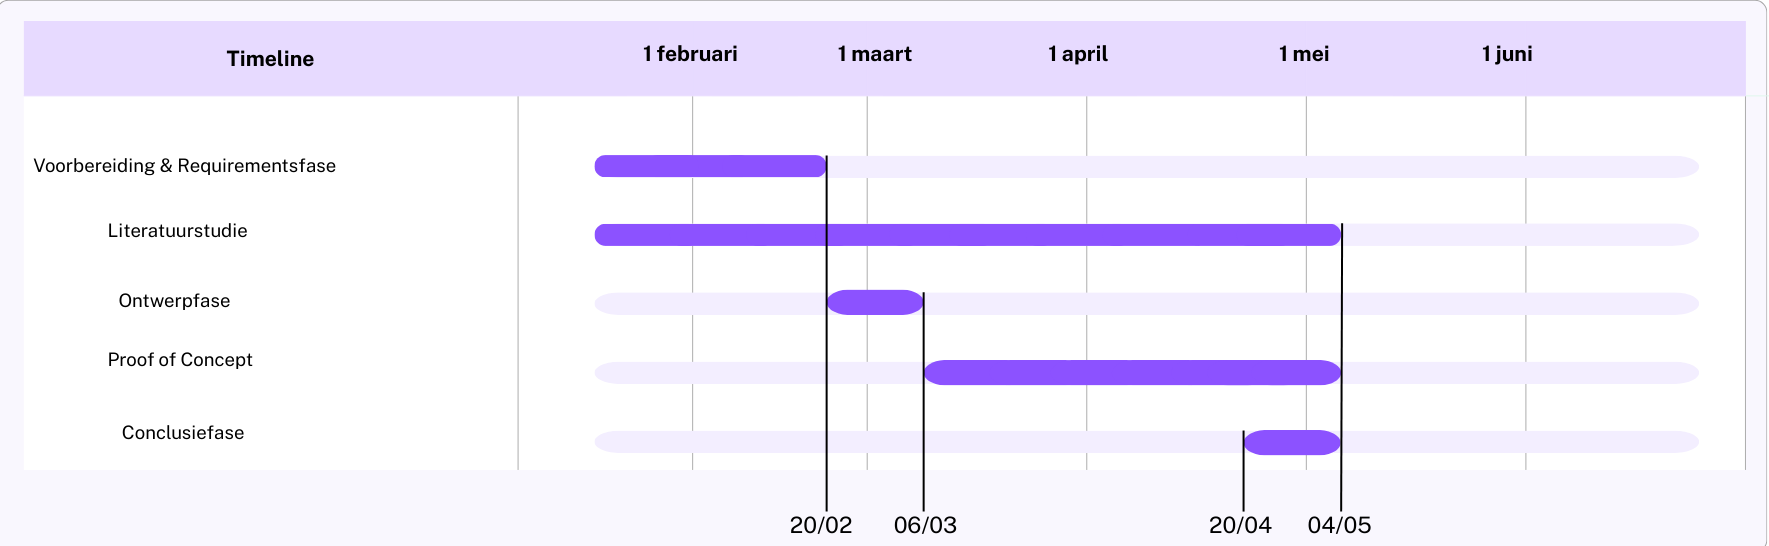
\includegraphics[width=.49\textwidth]{gantt_diagram.png}
    \caption{Tijdslijn bachelorproef CRA-compliance via CI/CD-pijplijn.}
    \label{fig:bp-tijdslijn}
\end{figure}
%---------- Verwachte resultaten ----------------------------------------------
\section{Verwacht resultaat, conclusie}%
\label{sec:verwachte_resultaten}

Het verwachte resultaat van deze bachelorproef is een volledig werkende CI/CD-pipeline die alle nodige securitytesten uit de shortlist uitvoert en een SBOM maakt en deze vergelijkt met een CVE-database waardoor de code volledig CRA-compliant is. Dit zorgt ervoor dat bekende en onbekende kwetsbaarheden opgespoord kunnen worden en gerapporteerd worden aan het development team zodat zij deze zo snel mogelijk kunnen oplossen. Hierdoor kan Excentis sneller en efficiënter inspelen op security-risico’s en wordt de kans verhoogd dat hun software tijdig voldoet aan de vereisten van de Cyber Resilience Act, waardoor ze een CE-label kunnen verkrijgen.

Deze bachelorproef biedt een meerwaarde voor zowel de development teams als het management team van Excentis. Voor de developers maakt het vinden van kwetsbaarheden eenvoudiger en sneller. Tegelijkertijd krijgt het management team inzicht in de algemene compliance-status van de softwareproducten.

Hoewel het doel is om een volledig werkende CI/CD-pipeline te hebben, kunnen er zich altijd problemen ontstaan. Bijvoorbeeld, bepaalde securitytools of SBOM-generators kunnen beperkingen hebben die de automatisatie voor een deel beïnvloeden. Mocht dit gebeuren, wordt er een duidelijke motivatie gegeven waarom de oorspronkelijke verwachtingen niet volledig overeenkomen met de gerealiseerde resultaten.



\printbibliography[heading=bibintoc]

\end{document}